\begin{frame}{Multi-messenger astronomy}
    \centering
    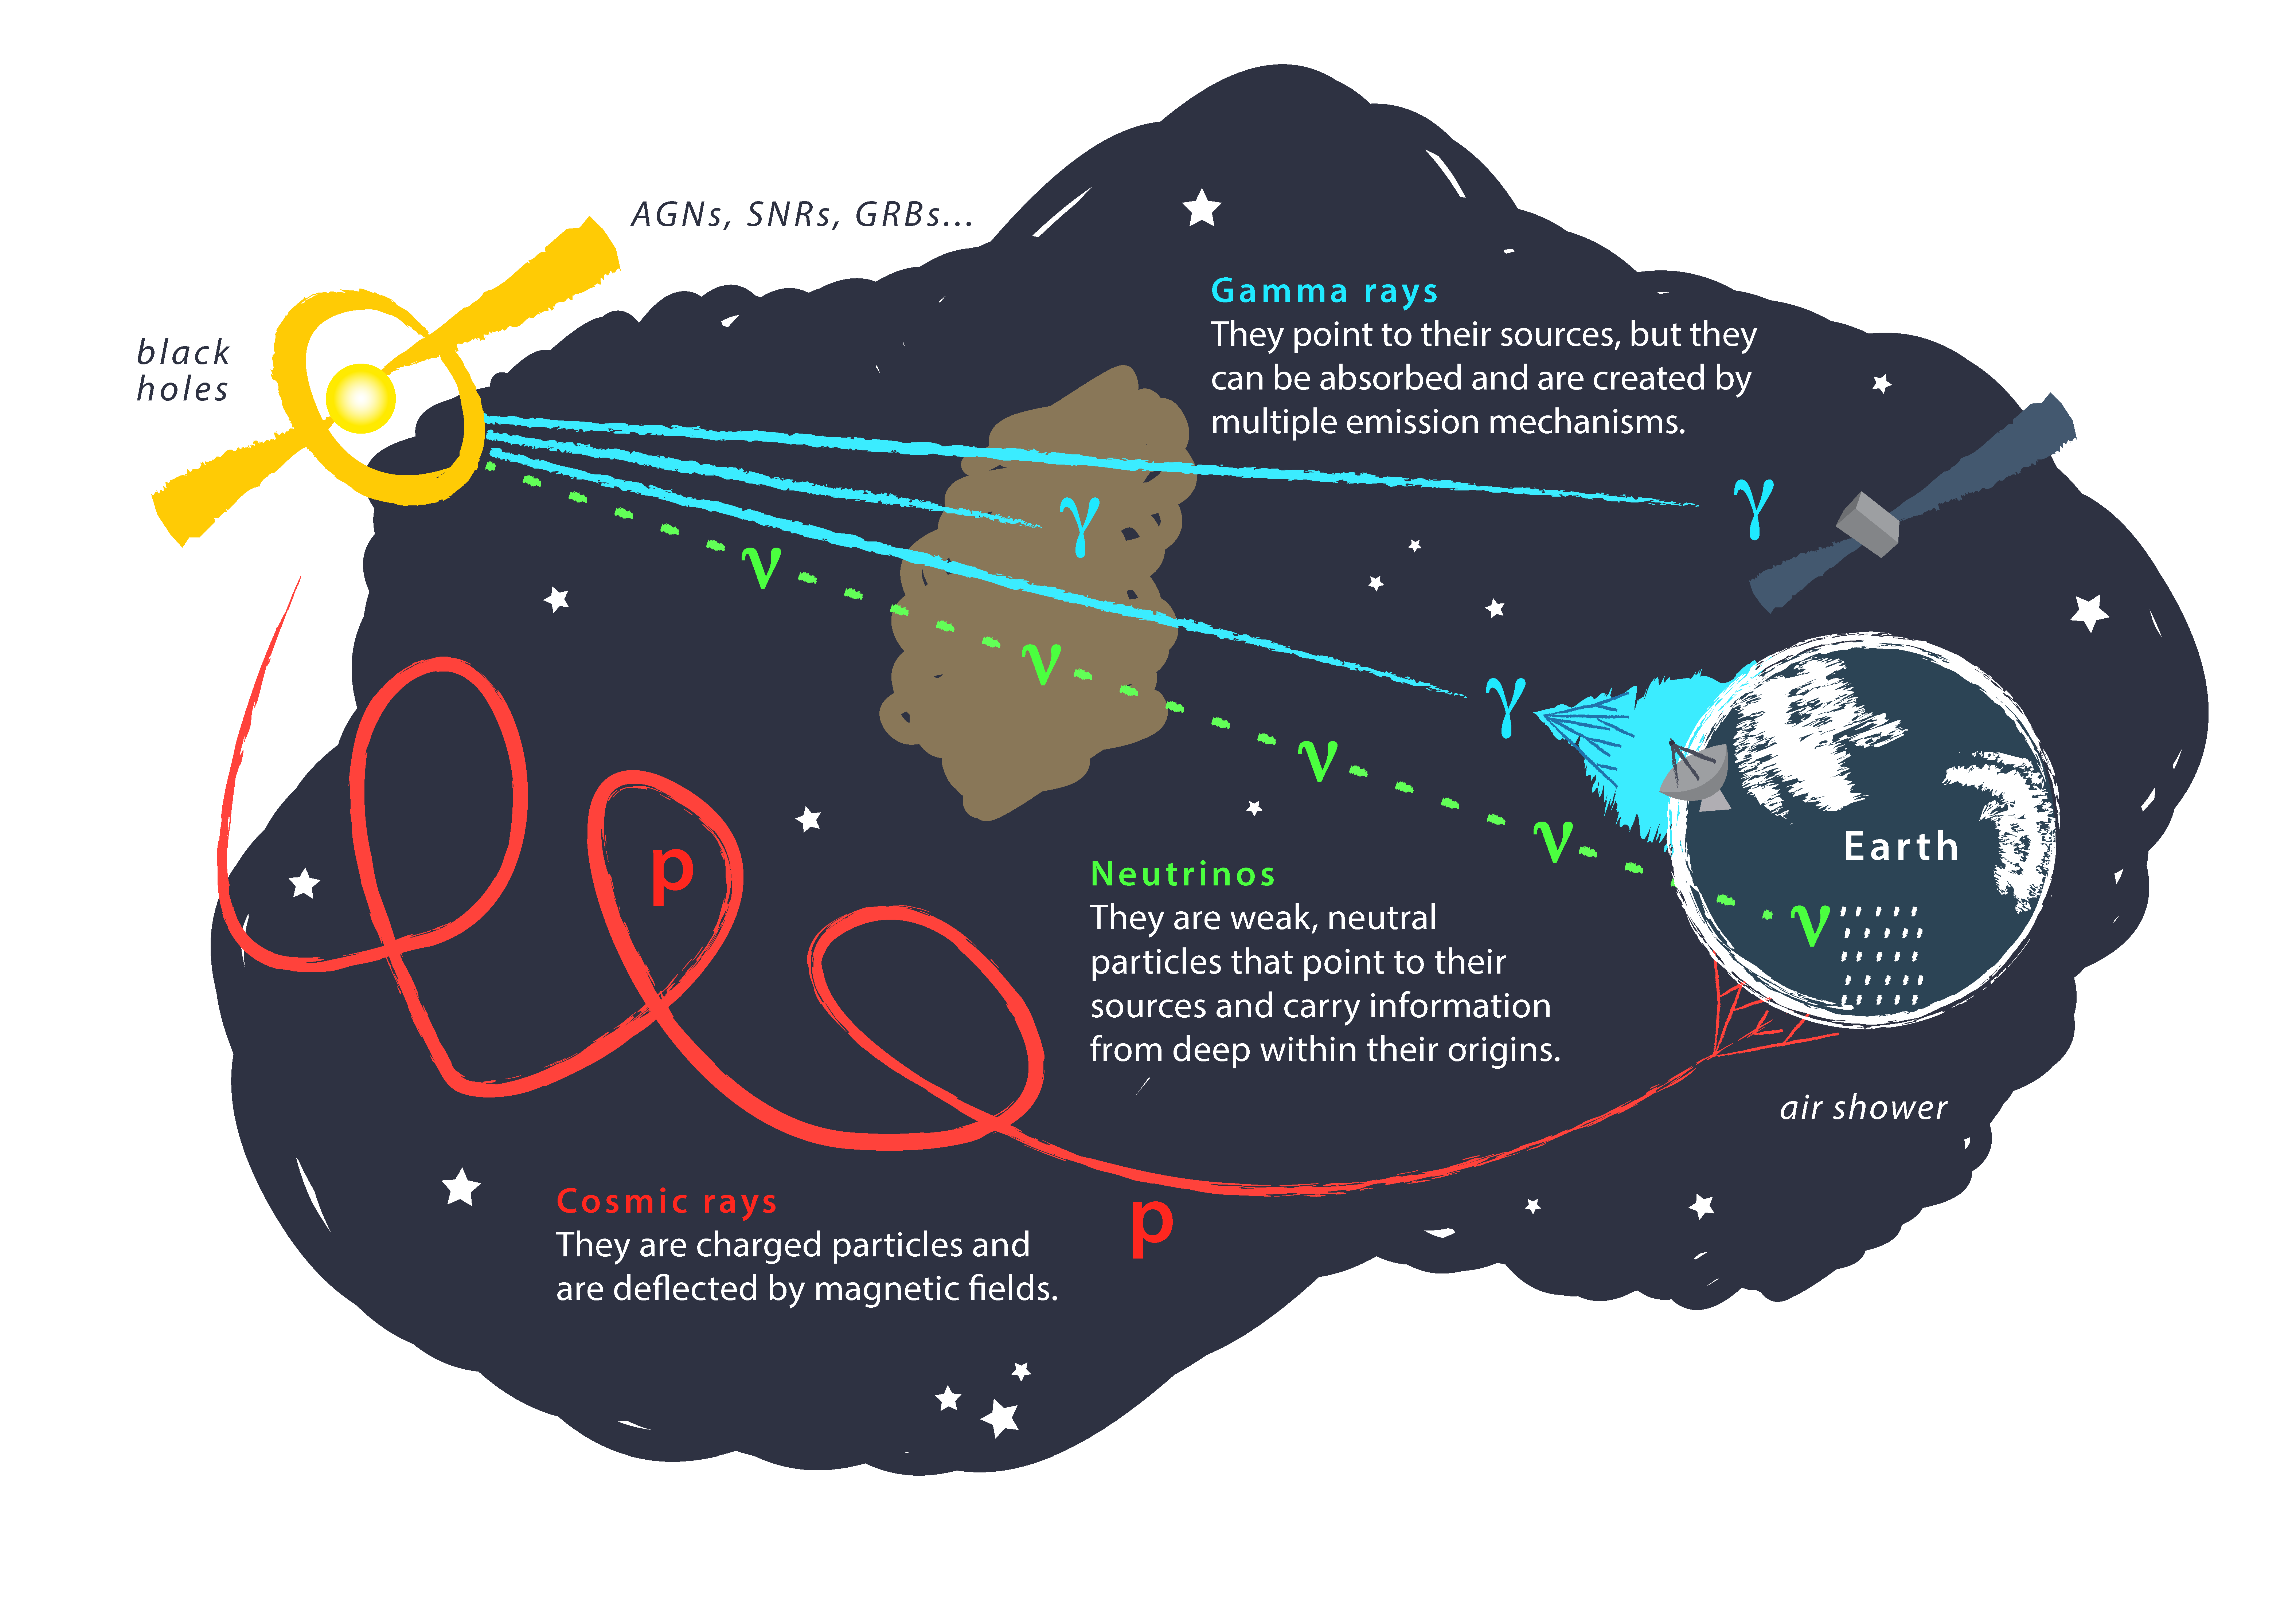
\includegraphics[width=0.75\textwidth]{images/cosmic_messengers.png}\\[-3.5\baselineskip]
    \hspace{4cm}[IceCube collaboration/ NSF]

    \note[item]{Verschiedene Botenteilchen von Quelle}
    \note[item]{Geladene Teilchen: Ablenkung}
    \note[item]{Nicht abgelenkt: Neutrinos \& Photonen}
    \note[item]{Neutrinos Nachteil: nur schwache WW $\to$ schwierige Detektion}
    \note[item]{Photonen: Absoption möglich \& direkt nur per Satellit}
    \note[item]{Luftschauer (Photonen und Protonen)}
\end{frame}

\begin{frame}{Extensive Air Showers}
    \centering
    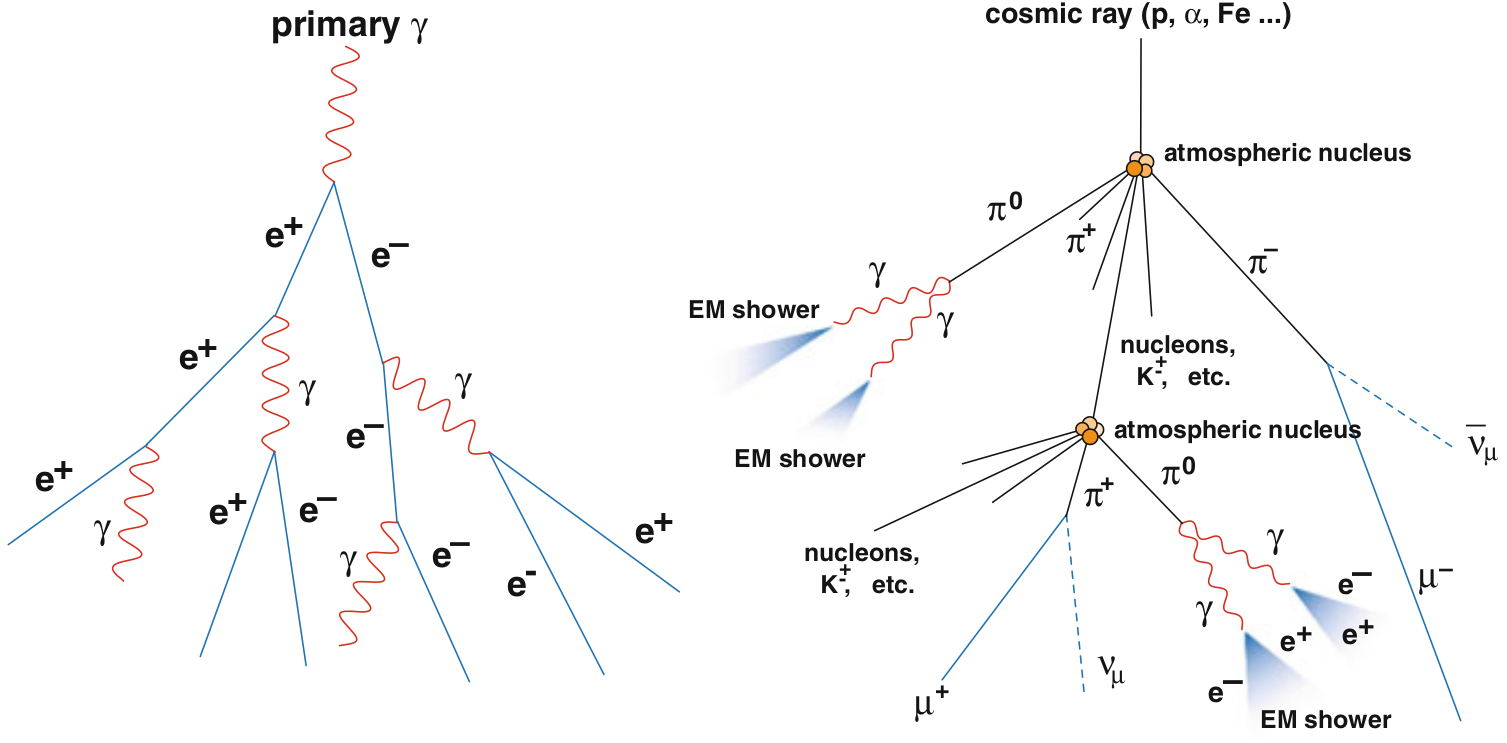
\includegraphics[width=\textwidth]{images/EAS.png}\\[-1.5\baselineskip]
    \hspace{-8cm}\href{https://www.jstor.org/stable/10.1086/522380}{[Robert M. Wagner, dissertation]}
    
    \note[item]{Photonen/ Gamma $\to$ Paarerzeugung \& Bremsstrahlung}
    \note[item]{Geladene Teilchen $\to$ starke WW $\to$ viele Prozesse}
    \note[item]{Geladene Teilchen schneller als Licht in Luft $\to$ Cherenkov Licht}
\end{frame}

\begin{frame}{The Imaging Air Cherenkov Technique}
    \centering
    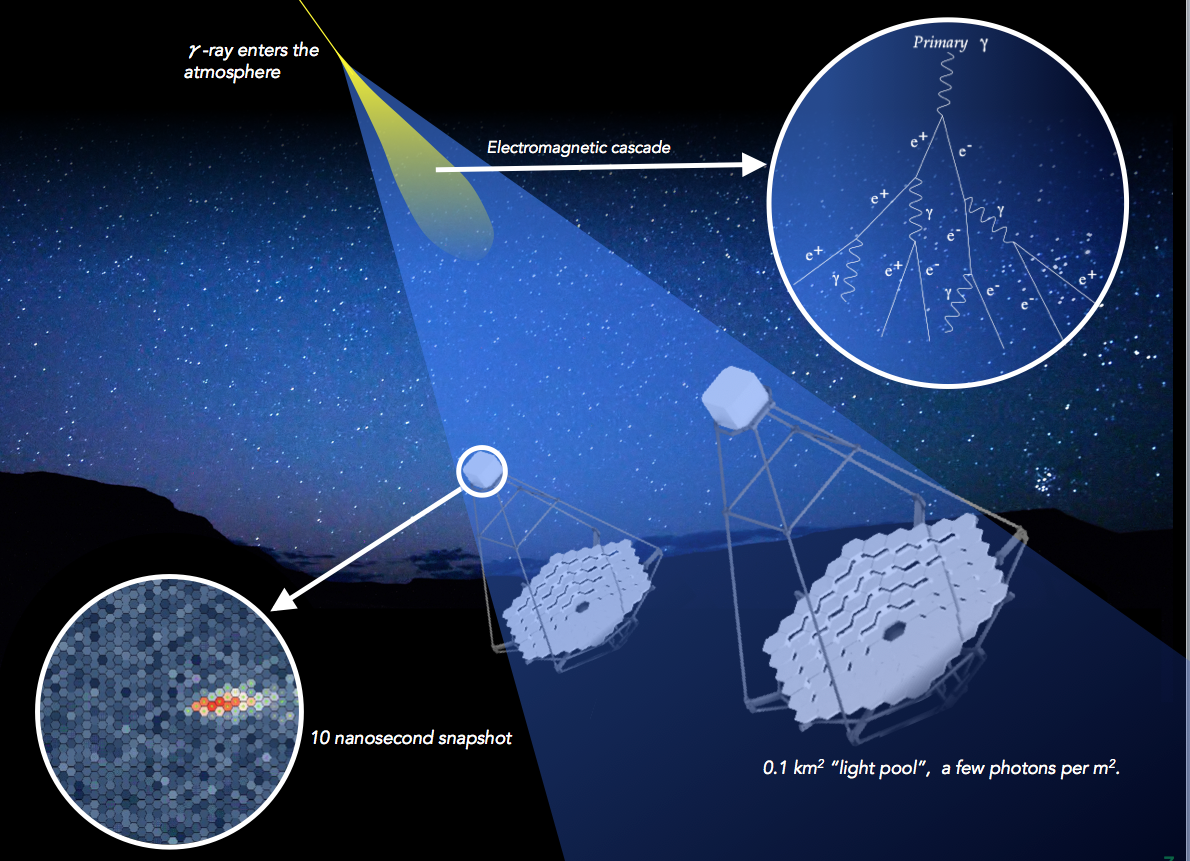
\includegraphics[width=0.64\textwidth]{images/Cherenkov-Effect.png}\\[-1.1\baselineskip]
    \small\href{https://www.cta-observatory.org/astri-detects-crab-at-tev-energies/}{\textcolor{white}{[cta-observatory.org]}}

    \note[item]{Cherenkov Licht in Kegel $\to$ Spiegel $\to$ Kamera}
    \note[item]{\enquote{Imaging Air Cherenkov Technik} \& Teleskope \enquote{Imaging Air Cherenkov Telescopes/ IACTs}}
\end{frame}

\begin{frame}{Observational strategy}
    \begin{columns}[onlytextwidth]
        \begin{column}{0.6\textwidth}
            Observe OFF region to estimate remaining background after gamma-hadron separation
            \begin{itemize}
                \item<1-> Independent observation
                    \begin{itemize}
                        \item[\textbf{\textcolor{tugreen}{\to}}] Less target observation time
                        \item[\textbf{\textcolor{tugreen}{\to}}] Possibly changed observation conditions
                    \end{itemize}
                \item<2-> Wobble mode
                    \begin{itemize}
                        \item Observe target with slight offset from camera center (LST-1: \SI{0.5}{\degree})
                        \item Camera geometry is radially symmetric $\to$ choose OFF regions along circle
                        \item[\textbf{\textcolor{tugreen}{\to}}] Maximise target observation time
                        \item[\textbf{\textcolor{tugreen}{\to}}] More OFF data
                    \end{itemize}
            \end{itemize}
        \end{column}
        \begin{column}{0.4\textwidth}
            \onslide<2->{
                \centering
                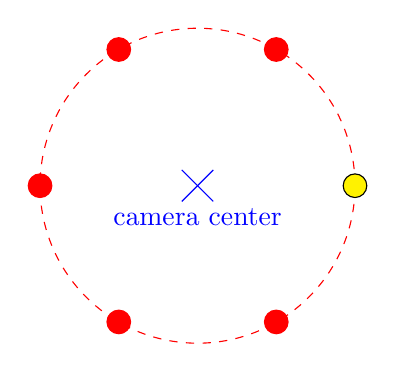
\begin{tikzpicture}
                    \draw[red, dashed] (0,0) circle (2);
                    \draw[blue] (-0.2,0.2) -- (0.2,-0.2);
                    \draw[blue] (0.2,0.2) -- (-0.2,-0.2);
                    \draw[blue] (0,-0.4) node {camera center};
                    \draw[fill=yellow] (2,0) circle (0.15);
                    \draw[red, fill=red] (1,1.73) circle (0.15);
                    \draw[red, fill=red] (-1,1.73) circle (0.15);
                    \draw[red, fill=red] (-2,0) circle (0.15);
                    \draw[red, fill=red] (-1,-1.73) circle (0.15);
                    \draw[red, fill=red] (1,-1.73) circle (0.15);
                \end{tikzpicture}
            }
        \end{column}
    \end{columns}

    \note[item]{Quelle beobachten}
    \note[item]{Selbst nach Hadronschauer Ausschluss $\to$ diffuses Hintergrund Signal}
    \note[item]{Quellsignal unterscheiden $\to$ Quellfreie OFF Region beobachten}
    \note[item]{Separat beobachten 
        \newline $\to$ Nachteile
    }
    \note<2->[item]{Alternative: wobble 
        \newline $\to$ Quelle mit Versatz
        \newline $\to$ Kamerageometrie Kreissymetrisch $\to$ OFF Regionen
        \newline $\to$ Vorteile
    }
\end{frame}